\mathchardef\mhyphen="2D
\documentclass[11pt]{article}
\usepackage[english]{babel}
\usepackage{minted}
\usepackage{amsfonts}
\usepackage{amsmath}
\usepackage{amsthm}
\usepackage{amssymb}
\usepackage{graphicx}
\usepackage{subcaption}
\usepackage[hypcap=false]{caption}
\usepackage{booktabs}
\usepackage[left=20mm, top=20mm, bottom=20mm, right=20mm]{geometry}
\usepackage{soul}
\usepackage{algorithm}
\usepackage{algpseudocode}
\usepackage[most]{tcolorbox}
\usepackage[colorlinks=true,linkcolor=darkcyan,filecolor=darkcerulean,urlcolor=magenta]{hyperref}
\usepackage{braket}
\usepackage{quantikz}

\newcommand{\calA}{\mathcal{A}}
\newcommand{\calB}{\mathcal{B}}
\newcommand{\calC}{\mathcal{C}}
\newcommand{\calD}{\mathcal{D}}
\newcommand{\calE}{\mathcal{E}}
\newcommand{\calF}{\mathcal{F}}
\newcommand{\calG}{\mathcal{G}}
\newcommand{\calH}{\mathcal{H}}
\newcommand{\calI}{\mathcal{I}}
\newcommand{\calJ}{\mathcal{J}}
\newcommand{\calK}{\mathcal{K}}
\newcommand{\calL}{\mathcal{L}}
\newcommand{\calM}{\mathcal{M}}
\newcommand{\calN}{\mathcal{N}}
\newcommand{\calO}{\mathcal{O}}
\newcommand{\calP}{\mathcal{P}}
\newcommand{\calQ}{\mathcal{Q}}
\newcommand{\calR}{\mathcal{R}}
\newcommand{\calS}{\mathcal{S}}
\newcommand{\calT}{\mathcal{T}}
\newcommand{\calU}{\mathcal{U}}
\newcommand{\calV}{\mathcal{V}}
\newcommand{\calW}{\mathcal{W}}
\newcommand{\calX}{\mathcal{X}}
\newcommand{\calY}{\mathcal{Y}}
\newcommand{\calZ}{\mathcal{Z}}

\newcommand{\bfA}{\mathbf{A}}
\newcommand{\bfB}{\mathbf{B}}
\newcommand{\bfC}{\mathbf{C}}
\newcommand{\bfD}{\mathbf{D}}
\newcommand{\bfE}{\mathbf{E}}
\newcommand{\bfI}{\mathbf{I}}
\newcommand{\bfS}{\mathbf{S}}
\newcommand{\bfP}{\mathbf{P}}
\newcommand{\bfQ}{\mathbf{Q}}
\newcommand{\bfU}{\mathbf{U}}
\newcommand{\bfv}{\mathbf{v}}
\newcommand{\bfu}{\mathbf{u}}
\newcommand{\bfdelta}{\mathbf{\Delta}}
\newcommand{\bfpi}{\mathbf{\Pi}}


\newcommand{\N}{\mathbb{N}}
\newcommand{\z}{\mathbb{Z}}
\newcommand{\I}{\mathbb{I}}
\newcommand{\C}{\mathbb{C}}

\newcommand{\keygen}{\mathsf{KeyGen}}
\newcommand{\enc}{\mathsf{Enc}}
\newcommand{\dec}{\mathsf{Dec}}
\newcommand{\negl}{\mathsf{negl}}
\newcommand{\commit}{\mathsf{Commit}}
\newcommand{\ccommit}{\mathsf{C\text{-}Commit}}

\newcommand{\setup}{\mathsf{Setup}}
\newcommand{\lsetup}{\mathsf{Setup\text{-}Lossy}}

\newcommand{\samplemat}{\mathsf{Sample\text{-}Dirac\text{-}Matrix}}
\newcommand{\eval}{\mathsf{Eval}}
\newcommand{\obf}{\mathsf{Obf}}

\newcommand{\phybb}[1]{p_{\mathrm{hyb}, #1}}
\newcommand{\lin}{\ell_{\mathrm{in}}}
\newcommand{\lout}{\ell_{\mathrm{out}}}
\newcommand{\bit}{\{0,1\}}
\newcommand{\sd}{\mathsf{SD}}
\newcommand{\lwe}{\mathsf{LWE}_{n,m,q,\chi}}
\newcommand{\sslwe}[4]{\mathsf{ss\text{-}LWE}_{#1,#2,#3,#4}}
\newcommand{\sslwec}{\sslwe{n}{m}{q}{\chi}}

\newcommand{\unif}[1]{\mathsf{Unif}_{\left[-#1, #1\right]}}
\newcommand{\func}[2]{\mathsf{Func}[#1, #2]}
\newcommand{\perm}[2]{\mathsf{Perm}[#1, #2]}
\newcommand{\ct}{\mathsf{ct}}
\newcommand{\Finverse}{F^{-1}}

\newcommand{\nqss}{\mathsf{No\mhyphen Query \mhyphen Semantic \mhyphen Security}}

\newcommand{\Tr}{\mathrm{Tr}}
\newcommand{\trace}[1]{\Tr\left( #1 \right)}

\newcommand{\prob}[1]{\Pr\left[ #1 \right]}

\newcommand{\ketbraa}[2]{\ket{#1}\bra{#2}}
\newcommand{\ketbra}[1]{\ketbraa{#1}{#1}}

\newcommand{\lddh}{\mathcal{L}_{DDH}}
\newcommand{\lnddh}{\mathcal{L}_{nDDH}}
\newcommand{\lddhkt}{\mathcal{L}_{DDH,k,t}}

\newlength{\protowidth}
\newcommand{\pprotocol}[4]{
{\begin{center}
\setlength{\protowidth}{\textwidth}
\addtolength{\protowidth}{-3\intextsep}

\fbox{
        \small
        \hbox{\quad
        \begin{minipage}{\protowidth}
    \begin{center}
    {\bf #1}
    \end{center}
        #4
        \end{minipage}
        \quad}
        }
        \captionof{figure}{\label{#3} #2}
\end{center}
} }

\newcommand{\defbox}[1]{
{\begin{center}
\setlength{\protowidth}{\textwidth}
\addtolength{\protowidth}{-3\intextsep}

\fcolorbox{darkcerulean}{cottoncandy}{
        \small
        \hbox{\quad
        \begin{minipage}{\protowidth}
    
        #1
        \end{minipage}
        \quad}
        }
\end{center}
        } }

\newcommand{\protocol}[4]{
\pprotocol{#1}{#2}{#3}{#4} }

\newtheorem{theorem}{Theorem}[section]
\newtheorem{claim}[theorem]{Claim}
\newtheorem{fact}[theorem]{Fact}
\newtheorem{definition}[theorem]{Definition}
\newtheorem*{answer}{Answer}
\newtheorem*{question}{Question}

\newtcolorbox{solution}[2][]{every float=\centering,breakable,enhanced,adjusted title={#2},colback=codegray,colframe=codegray!50!black}

\linespread{1.0}

\definecolor{codegray}{rgb}{0.98,0.97,0.93}
\definecolor{cottoncandy}{rgb}{1.0, 0.84, 0.95}
\definecolor{darkcerulean}{rgb}{0.03, 0.27, 0.49}
\definecolor{darkcyan}{rgb}{0.0, 0.50, 0.45}

\title{ECE 382V: Introduction to Quantum Computing Systems from a Software and Architecture Perspective\\Lab 2}
\author{Sayam Sethi}
\date{November 2023}

\begin{document}

\maketitle

\tableofcontents

\section{Introduction}
In this lab we implement and understand the different Quantum Error Correction techniques starting from the $3$-qubit repetition code and moving onto the distance $3$ surface codes. We aim to better comprehend the pros and cons of the different techniques and why they are used/not used anymore.

\section{The Repetition Code}

\subsection{$3$-Qubit Repetition}
\subsubsection{Bit Flip and Phase Flip Errors}
The error correction scheme used for handling bit flip and phase flip erorrs is almost the same, the only difference between the two is the logical states that the two qubits are entangled in. The bit-flip entanglement is in the standard basis and hence the logical states are $\ket{000}, \ket{111}$ however, the logical states for the phase flip are $\ket{+++}, \ket{---}$. The two circuits are shown in Figure~\ref{fig:3}.
\begin{figure}[h!]
    \begin{subfigure}{\linewidth}
        \includegraphics[width=\linewidth]{outputs/bit_3.png}
        \caption{The error correction circuit for the bit flip error}
    \end{subfigure}
    \begin{subfigure}{\linewidth}
        \includegraphics[width=\linewidth]{outputs/phase_3.png}
        \caption{The error correction circuit for the phase flip error}
    \end{subfigure}
    \caption{The circuits for the bit flip and the phase flip repetition codes. The region between the first two barriers is where the gate operations are done and where the errors can be injected.}\label{fig:3}
\end{figure}

The decoder for both the circuits looks exactly the same as can be seen in Figure~\ref{fig:3}. The only difference is in the decoding applied for the respective value of the decoder, in the case of a bit flip error, the $\mathbf{X}$ gate is applied and in the case of the phase flip error, the $\mathbf{Z}$ gate is applied. On running the statevector simulations on this circuit, it can be seen that the errors injected are always corrected successfully, and the result of measuring $q_0$ is always $0$.

\subsubsection{Measurement Error}
On running the circuits on a noisy simulation (IBM FakeKolkataV2), we notice that the errors are not always successfully corrected. The success rate is around $95\%$ as can be seen from the following plots,
\begin{figure}[h!]
    \begin{subfigure}{0.5\linewidth}
        \includegraphics[width=\linewidth]{outputs/measure_3_none.png}
        \caption{Plot for the measurement with no errors}
    \end{subfigure}
    \begin{subfigure}{0.5\linewidth}
        \includegraphics[width=\linewidth]{outputs/measure_3_0.png}
        \caption{Plot for the measurement with bit-flip on $q_0$}
    \end{subfigure}
    \begin{subfigure}{0.5\linewidth}
        \includegraphics[width=\linewidth]{outputs/measure_3_1.png}
        \caption{Plot for the measurement with bit-flip on $q_1$}
    \end{subfigure}
    \begin{subfigure}{0.5\linewidth}
        \includegraphics[width=\linewidth]{outputs/measure_3_2.png}
        \caption{Plot for the measurement with bit-flip on $q_2$}
    \end{subfigure}
    \caption{Plots for the different error introduced manually when running on a noisy simulator.}\label{fig:3_measure}
\end{figure}

As can be seen from the plots (Figure~\ref{fig:3_measure}), the decoding success rate decreases when the syndrome values read more $1$'s. However, the success rate is still quite high.

\subsection{$5$-Qubit Repetition}
\subsubsection{Bit Flip and Phase Flip Errors}
The error correction scheme used for handling bit flip and phase flip erorrs is almost the same, the only difference between the two is the logical states that the two qubits are entangled in. The bit-flip entanglement is in the standard basis and hence the logical states are $\ket{00000}, \ket{11111}$ however, the logical states for the phase flip are $\ket{+++++}, \ket{-----}$. The two circuits are shown in Figure~\ref{fig:5}.
\begin{figure}[h!]
    \begin{subfigure}{\linewidth}
        \includegraphics[width=\linewidth]{outputs/bit_5.png}
        \caption{The error correction circuit for the bit flip error}
    \end{subfigure}
    \begin{subfigure}{\linewidth}
        \includegraphics[width=\linewidth]{outputs/phase_5.png}
        \caption{The error correction circuit for the phase flip error}
    \end{subfigure}
    \caption{The circuits for the bit flip and the phase flip repetition codes. The region between the first two barriers is where the gate operations are done and where the errors can be injected.}\label{fig:5}
\end{figure}

The decoder for both the circuits looks exactly the same as can be seen in Figure~\ref{fig:5}. The only difference is in the decoding applied for the respective value of the decoder, in the case of a bit flip error, the $\mathbf{X}$ gate is applied and in the case of the phase flip error, the $\mathbf{Z}$ gate is applied. On running the statevector simulations on this circuit, it can be seen that the errors injected are always corrected successfully, and the result of measuring $q_0$ is always $0$.

\subsubsection{Measurement Error}
On running the circuits on a noisy simulation (IBM FakeKolkataV2), we notice that the errors are not always successfully corrected. The success rate varies significantly (between $77\%$ and $88\%$) as can be seen from the following plots,
\begin{figure}[h!]
    \begin{subfigure}{0.5\linewidth}
        \includegraphics[width=\linewidth]{outputs/measure_5_none.png}
        \caption{Plot for the measurement with no errors}
    \end{subfigure}
    \begin{subfigure}{0.5\linewidth}
        \includegraphics[width=\linewidth]{outputs/measure_5_0.png}
        \caption{Plot for the measurement with bit-flip on $q_0$}
    \end{subfigure}
    \begin{subfigure}{0.5\linewidth}
        \includegraphics[width=\linewidth]{outputs/measure_5_1.png}
        \caption{Plot for the measurement with bit-flip on $q_1$}
    \end{subfigure}
    \begin{subfigure}{0.5\linewidth}
        \includegraphics[width=\linewidth]{outputs/measure_5_2.png}
        \caption{Plot for the measurement with bit-flip on $q_2$}
    \end{subfigure}
    \begin{subfigure}{0.5\linewidth}
        \includegraphics[width=\linewidth]{outputs/measure_5_3.png}
        \caption{Plot for the measurement with bit-flip on $q_3$}
    \end{subfigure}
    \begin{subfigure}{0.5\linewidth}
        \includegraphics[width=\linewidth]{outputs/measure_5_4.png}
        \caption{Plot for the measurement with bit-flip on $q_5$}
    \end{subfigure}
    \caption{Plots for the different error introduced manually when running on a noisy simulator.}\label{fig:5_measure}
\end{figure}

As can be seen from the plots (Figure~\ref{fig:5_measure}), the decoding success rate decreases when the syndrome values read more $1$'s. However, compared to the success rate of the 3 qubit repetition code, the success rate is much lower due to the increased gate errors.

\section{Surface Codes}

\subsection{Circuit Creation}
The rotated surface code for distance three was implemented using the circuit show in Figure~\ref{fig:surface}. Two rounds of syndrome extraction are done. The first one is used to entangle the data qubits and to obtain the reference syndrome. The second round is used to compare the newly obtained syndrome with the reference syndrome. The \texttt{xor} between the two syndromes can then be used to determine the correction to be applied by using it as the input to the decoder. Finally, the correction is applied (not shown in the figure) and another round of syndrome extraction is done to see if the syndrome has been corrected (again, not shown in the figure). This surface code implementation is capable of correcting up to one bit-flip and one phase-flip error simultaneously on any of the data qubits.
\begin{figure}[h!]
    \centering
    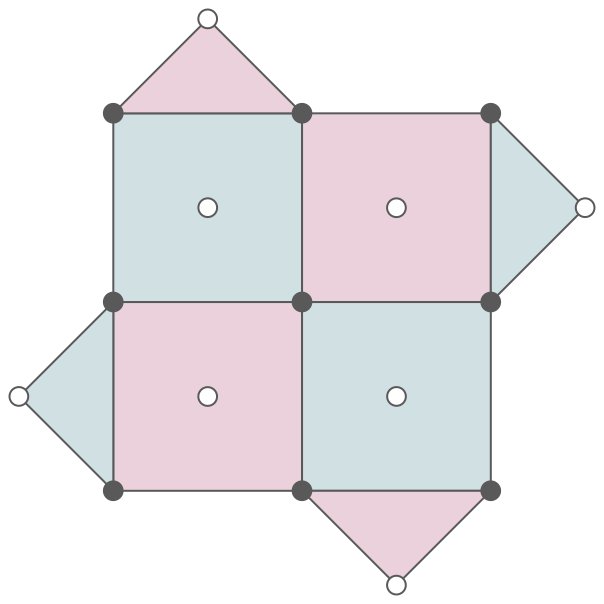
\includegraphics[width=\linewidth]{outputs/surface_code.png}
    \caption{The circuit for the surface code. The region between the two syndrome extraction regions is where the gate operations are done and where the errors can be injected.}\label{fig:surface}
\end{figure}

\subsection{Decoder Implementation}
A static decoder was implemented by using the \texttt{xor} values between the two syndrome results as the input to the decoder. If the decoder had already been mapped to some error, the error was updated. Since we only want to correct up to one bit flip and one phase flip errors, we can have at most $100$ errors ($10$ possibilities for each: error on one of the $9$ data qubits + no error). However, since we only have $8$ bits for the syndrome, we can only store the decoding for up to $64$ errors, thus overwriting $36$ decoding. The decoding is shown below,
\inputminted{python}{outputs/surface_code_decoder}

\subsection{Error Correction}
Now that we have the decoder, the error correction circuit is designed by performing controlled CNOT based on all possible initial syndromes and their \texttt{xor} values. Since this leads to a very large circuit, the circuit could not be shown. However, on running the circuit on all possible $100$ error scenarios, it was observed that the syndrome is restored to what we started off with. This happens even when the error correction is different from the one that was actually injected. The reason for this is that the correction applied actually inserts even more errors and thus the syndrome is restored, however, the resultant circuit is actually erroneous. However, since this only happens on the boundary qubits, this can be corrected if we insert more syndrome qubits on the boundaries. However, since this wasn't the goal of the lab, this wasn't done.

\subsection{Measurement Error}
Since the circuit obtained after implementing the error correction was very big, it could not be run on the noisy simulator in finite time. Therefore, to simulate the measurement errors, the correction circuit was instead modified to read a different syndrome than what it should have been. This was done by changing the \texttt{xor} values between the two syndromes. The results are shown below,
\inputminted{python}{outputs/surface_code_measure}

The above output log can be read as, the first list is the bit flip error injected, the second list is the phase flip error injected, the first $8$-bit input syndrome is the reference syndrome, the next $8$ bit input is the syndrome obtained after the error was injected (without the measurement error), the last $8$ bits are the syndrome obtained after the error correction was applied. It can be observed that the measurement error remains in the final syndrome for most of the corrections. It propagates even further when the incorrect correction was applied.

\section{Conclusion}
It can be seen that the error correction techniques are very helpful in mitigating the errors that occur because of noisy simulations. However, they are still tedious to implement and we still have a long way to go before we can implement successful error correction schemes in a real quantum system.

\end{document}